\documentclass[a4paper,10pt,twocolumn,uplatex]{jsarticle}
\usepackage{style/nislab,style/resume}

%---------------------------------------------------------------------
% レジュメ種別・日付設定(要変更)
% \type{} 1:修士論文諮問会 2:卒業論文発表会 3:月例発表会 4:研究室合同発表会
%---------------------------------------------------------------------
\type{3}
\year{2022}
\month{6}
\date{11}

%---------------------------------------------------------------------
% ページ番号設定(要変更)
%---------------------------------------------------------------------
\setcounter{page}{9}

%---------------------------------------------------------------------
% 変更不要
%---------------------------------------------------------------------
\begin{document}

%---------------------------------------------------------------------
% タイトル作成部分(要変更)
% \maketitle{タイトル}{title}{名前}{name}
%---------------------------------------------------------------------
\maketitle{IoTデバイスの通信セキュリティ向上のための\\ホームネットワーク仮想化フレームワークの提案}
{Proposal of Home Network Virtualization Framework\\to Improve Communication Security of IoT Devices}
{塚崎 拓真}
{Takuma Tsukasaki}

%---------------------------------------------------------------------
\section{はじめに}
近年,IoT(Internet of Things)の可能性が注目され,今後あらゆるモノがネットワークに接続され,利用されることが予想される.
しかし,IoTの発展により利便性が高まる一方で,従来ネットワークに接続されていなかったモノが接続されることにより,セキュリティ上のリスクも高まっている\cite{security}.
IoTデバイスは,十分なセキュリティを考慮せずに開発されたものが多く,脆弱なパスワードによる侵入やプライバシー保護の不十分さ等のセキュリティ対策不足が顕著である\cite{owasp}.そのため,悪意のある攻撃者によるサイバー攻撃の標的になりやすい.
また,今後はホームネットワーク内で閉じたデバイス間の通信によって連携を行う形になることが想定され\cite{d2d},各デバイスにおいてアクセス制御等の更なるセキュリティ対策を行う必要がある.\par
そこで本研究では,コンテナ上にセキュリティ対策を施したProxyを作成し,IoTデバイスに対して,仮想的にセキュリティ対策を適用するシステムを提案する.また,SDN(Software Defined Networks)の代表的プロトコルであるOpenFlowを用いて,ホームネットワーク内の通信を監視するフレームワークの構築も検討する.


\begin{figure}[!tb]
  \centering
  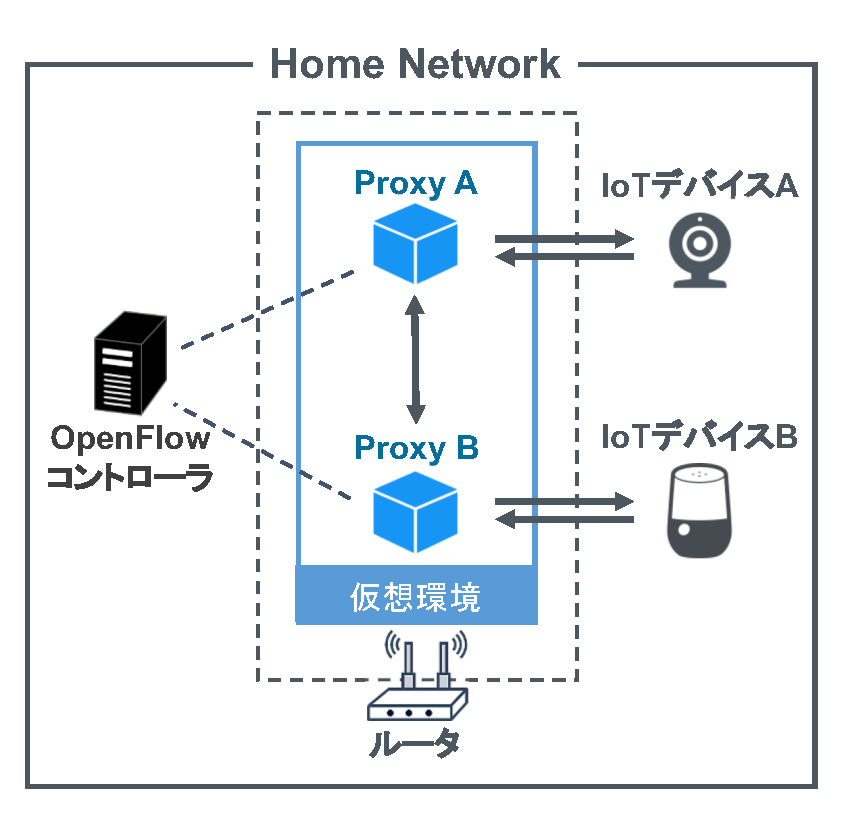
\includegraphics[width=\linewidth]{img/system.eps}
  \caption{提案システムの構成}
  \label{fig:system}
\end{figure}

%---------------------------------------------------------------------
\section{提案システム}
\subsection{システム構成}
提案システムの構成を図\ref{fig:system}に示し,詳細を以下に示す.本提案システムは,IoTデバイス,Proxy,ルータ,OpenFlowコントローラから構成される.
\begin{itemize}
  \item \underline{IoTデバイス}\mbox{}\\
        本研究で扱うIoTデバイスは,CPU等のリソースを十分に保持しておらず,直接セキュリティ対策を適用できないデバイスと定義する.
  \item \underline{Proxy}\mbox{}\\
        IoTデバイスに要求されるセキュリティ対策を,コンテナ上で実現したものである.そして,IoTデバイスからの通信を中継し,セキュリティ対策を適用する.各IoTデバイスに必要なセキュリティ対策をそれぞれ作成,適用することで,対象デバイスに応じた必要なセキュリティ対策を実現できる.
  \item \underline{ルータ}\mbox{}\\
        IoTデバイス間通信の中継機器として用いる.ルータ上にProxyの実行環境を生成する.Proxyが作成される際に必要とされるリソースを提供することが可能である.
  \item \underline{OpenFlowコントローラ}\mbox{}\\
        Proxy内に作成されたOpenFlowスイッチと通信を行い,ホームネットワーク内の通信を監視する.ホームネットワーク内部に設置する.
\end{itemize}

\begin{figure*}[!tb]
  \centering
  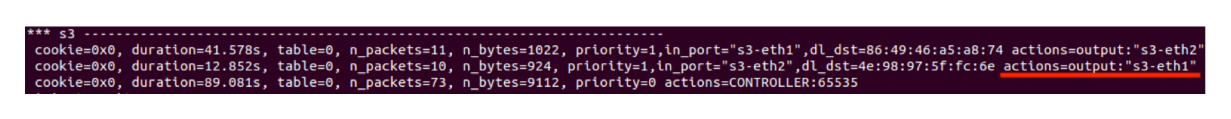
\includegraphics[width=\linewidth]{img/result_flow4v3.eps}
  
\includegraphics[width=\linewidth]{img/result_flow2v3.eps}
  
\includegraphics[width=\linewidth]{img/result_flow3v2.eps}
  \caption{登録済みのホストのフローテーブル(上),異常時のパケットをDrop処理するフローテーブル(中),その後のアクションが削除されたフローテーブル(下)}
  \label{fig:result1}
\end{figure*}

\subsection{Proxyのセキュリティ対策}
本研究におけるセキュリティ対策は,Proxyごとに異なるセキュリティ対策を適用可能である.これにより,リソース制限が原因でIoTデバイスに直接適用できないセキュリティ対策を適用できる.
また,様々なハードウェアやアプリケーションへの適用や,様々なセキュリティ要件の変更に対しても柔軟に対応が可能となる.\par
コンテナ上で作成されるセキュリティ対策は,各セキュリティ対策に対応したコンテナのimageファイルで定義される.IoTデバイスに適用したいセキュリティ対策が複数ある場合においても,対象デバイスの規格に対応したセキュリティ対策をそれぞれ作成し,ソフトウェアモジュールのような形で組み合わせて定義することで,imageファイルを作成することが可能となる.

\subsection{OpenFlowによるフローチェック}
本研究におけるネットワーク監視をOpenFlowを用いて行う.一つのIoTデバイスに対し,コンテナ上にOpenFlowスイッチの機能を生成する.IoTデバイスは,このOpenFlowスイッチを中継し,デバイス間通信を行う.OpenFlowコントローラは事前にIoTデバイスの情報を保持しており,OpenFlowスイッチとの通信が確立でき次第,デバイス間通信のフローテーブルを作成する.ホームネットワークの特性である各IoTデバイスのトラフィック情報は既知であることや,変化が大きくないことを考慮し,IPアドレスや通信頻度の確認を行い,フローレベルにおける異常の検知を行う.
% 異常を検知した場合は,そのパケットのDrop処理を指示したフローテーブルに変更し,その後フローテーブルを削除する.また同時に,ユーザへ異常検知を通知する.


%---------------------------------------------------------------------
\section{シミュレーション実験}
% \subsection{実装環境}
% Proxyは,Dockerを用いて作成した.Dockerで作成されるコンテナ上でProxyを稼働させることで,複数のProxyをリソースやオーバーヘッドを抑えて作成できる.また,これらのProxyは,Docker Hubより配布されるDocker Imageを用いることで容易に作成できる.また,OpenFlowコントローラは,SDNを実現するための開発フレームワークであるRyuを用いて作成した.

\subsection{評価内容}
本研究の評価として,まずセキュリティ対策が適用されているかを検証した.今回の異常通信としては,登録されていないIoTデバイスから通信があった場合と,あるデイバイスからの通信頻度が通常と異なる場合を想定した.その状況において,コンテナ上で作成したOpenFlowによるフローチェックが行われているかを検証した.\par
また,提案システムの有効性を示すため,提案システムを適用した上で,IoTデバイス間通信を20回行なった際のラウンドトリップタイムを計測した.比較対象として,セキュリティ対策を適用せず,ルータを経由してデバイス間通信を行う場合についても計測を行った.

% \begin{figure}[!tb]
%   \centering
%   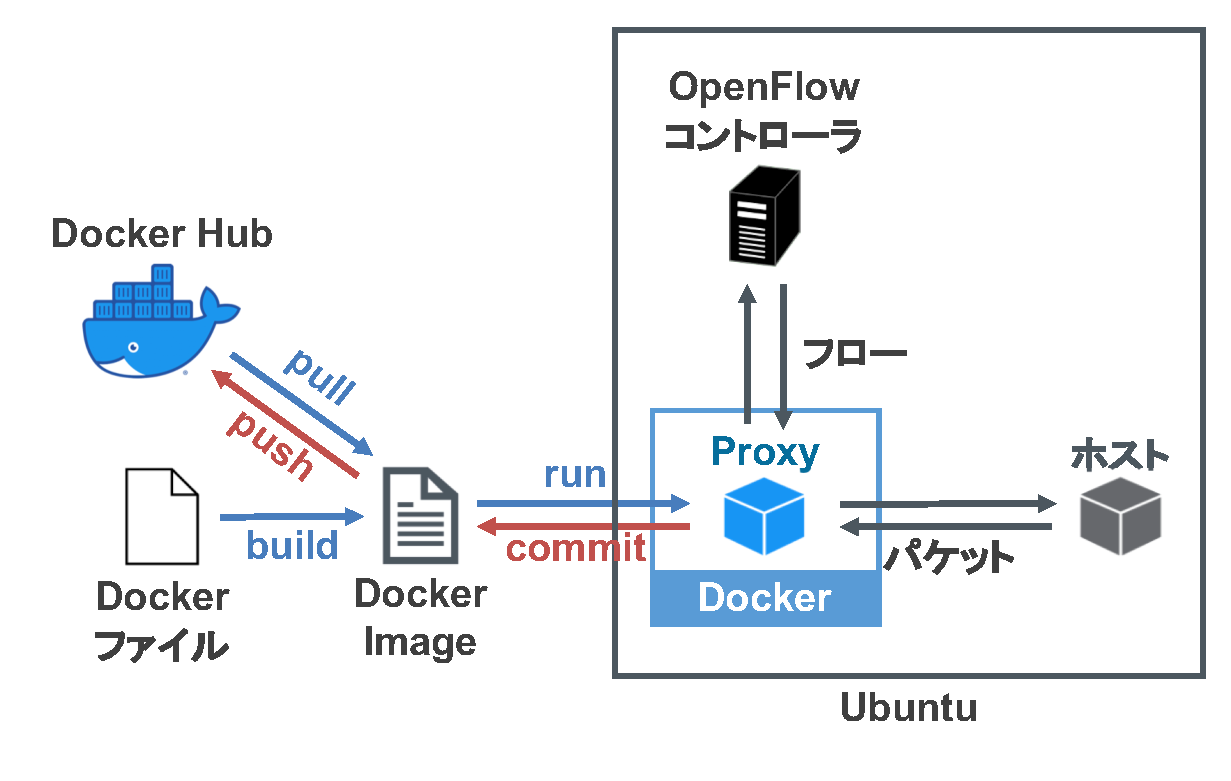
\includegraphics[width=\linewidth]{img/program.eps}
%   \caption{実装環境の構成}
%   \label{fig:program}
% \end{figure}


\subsection{評価環境}
今回のシミュレーション実験においては,IoTデバイスや通信に関するログの収集・出力機能を実装し,セキュリティ対策として適用した.また,OpenFlowスイッチのイメージも取得し,OpenFlowによるフローチェックも行った.事前に2台のホストを設置した環境に,新たに1台ホストを追加し,そのホストが通信要求を行う環境を作成した.
ProxyはDockerを,OpenFlowコントローラはRyuを用いて作成した.


\subsection{評価結果}
登録済みのIoTデバイスから通信要求が来た場合,登録していないIoTデバイスや,通常の通信頻度と異なる等の異常の通信がなされている場合のフローテーブルの結果を図\ref{fig:result1}に示す.通常時は他のデバイスに対し,通信を許可するフローテーブルが作成されている.一方で,異常時はパケットをDrop処理するフローテーブルが作成されており,その後,そのフローテーブルが削除されていることがわかる.\par
また,提案システムは,セキュリティ対策を施していないシステムにおける通信より,ラウンドトリップタイムの平均値が約1.06ms,最大値が約10.62ms大きくなった.


%---------------------------------------------------------------------
\section{まとめ}
本研究では,IoTのセキュリティ上のリスクにおいて,今後,ホームネットワーク内で閉じたデバイス間通信が多くなり,各IoTデバイスにおいてアクセス制御等の更なるセキュリティ対策を行う必要があることに注目した.
そこで,コンテナを用いたIoTデバイスへのセキュリティ対策の適用と,OpenFlowを用いたホームネットワーク監視を行うフレームワークの構築を提案した.
そして,IoTデバイス間で閉じた通信を行うシミュレーション評価の比較を行い,提案システムはホームネットワークにおいてセキュリティ要件を保つことと,通信性能も許容範囲であることを示した.

%---------------------------------------------------------------------
% Bibliography(参考文献)
%---------------------------------------------------------------------
% thebibliography を利用する場合は以下を使用
\footnotesize{
  \begin{thebibliography}{99}
    \bibitem{security} 総務省:IoT・5Gセキュリティ総合対策2020,総務省(オンライン),
    \url{https://www.soumu.go.jp/main_content/000698567.pdf}(参照 2022-03-28).
    \bibitem{owasp} Ferrara, P., Mandal, A.K., Cortesi, A. and Spoto, F.: Static analysis for discovering IoT vulnerabilities, International Journal on Software Tools for Technology Transfer, Vol.23, No.1, pp.71-88(2021).
    \bibitem{d2d} Pawar, P. and Trivedi, A.: Device-to-Device Communication Based IoT System: Benefits and Challenges, IETE Technical Review, Vol.36, No.4, pp.362-374(2019).
  \end{thebibliography}
}

% BibTex を利用する場合は以下を使用(初めての人には難しいかも)
% \bibliographystyle{junsrt}
% \bibliography{myref}

%---------------------------------------------------------------------
\end{document}
%---------------------------------------------------------------------
